% this is a simplified version of 
% https://github.com/yihui/knitr/blob/master/inst/examples/knitr-beamer.Rnw
\documentclass{beamer}\usepackage[]{graphicx}\usepackage[]{color}
%% maxwidth is the original width if it is less than linewidth
%% otherwise use linewidth (to make sure the graphics do not exceed the margin)
\makeatletter
\def\maxwidth{ %
  \ifdim\Gin@nat@width>\linewidth
    \linewidth
  \else
    \Gin@nat@width
  \fi
}
\makeatother

\definecolor{fgcolor}{rgb}{0.345, 0.345, 0.345}
\newcommand{\hlnum}[1]{\textcolor[rgb]{0.686,0.059,0.569}{#1}}%
\newcommand{\hlstr}[1]{\textcolor[rgb]{0.192,0.494,0.8}{#1}}%
\newcommand{\hlcom}[1]{\textcolor[rgb]{0.678,0.584,0.686}{\textit{#1}}}%
\newcommand{\hlopt}[1]{\textcolor[rgb]{0,0,0}{#1}}%
\newcommand{\hlstd}[1]{\textcolor[rgb]{0.345,0.345,0.345}{#1}}%
\newcommand{\hlkwa}[1]{\textcolor[rgb]{0.161,0.373,0.58}{\textbf{#1}}}%
\newcommand{\hlkwb}[1]{\textcolor[rgb]{0.69,0.353,0.396}{#1}}%
\newcommand{\hlkwc}[1]{\textcolor[rgb]{0.333,0.667,0.333}{#1}}%
\newcommand{\hlkwd}[1]{\textcolor[rgb]{0.737,0.353,0.396}{\textbf{#1}}}%
\let\hlipl\hlkwb

\usepackage{framed}
\makeatletter
\newenvironment{kframe}{%
 \def\at@end@of@kframe{}%
 \ifinner\ifhmode%
  \def\at@end@of@kframe{\end{minipage}}%
  \begin{minipage}{\columnwidth}%
 \fi\fi%
 \def\FrameCommand##1{\hskip\@totalleftmargin \hskip-\fboxsep
 \colorbox{shadecolor}{##1}\hskip-\fboxsep
     % There is no \\@totalrightmargin, so:
     \hskip-\linewidth \hskip-\@totalleftmargin \hskip\columnwidth}%
 \MakeFramed {\advance\hsize-\width
   \@totalleftmargin\z@ \linewidth\hsize
   \@setminipage}}%
 {\par\unskip\endMakeFramed%
 \at@end@of@kframe}
\makeatother

\definecolor{shadecolor}{rgb}{.97, .97, .97}
\definecolor{messagecolor}{rgb}{0, 0, 0}
\definecolor{warningcolor}{rgb}{1, 0, 1}
\definecolor{errorcolor}{rgb}{1, 0, 0}
\newenvironment{knitrout}{}{} % an empty environment to be redefined in TeX

\usepackage{alltt}
\IfFileExists{upquote.sty}{\usepackage{upquote}}{}
\begin{document}
%\SweaveOpts{concordance=TRUE}

\title{Introducci\'on a la Gen\'omica \\ UNAL nov 2017}
\author{Alejandro Caceres \\ ISGlobal, Barcelona}


\maketitle

% very important to use option [fragile] for frames containing code output!

\begin{frame}[fragile]
\frametitle{Gen\'omica}

Estudio de la biolo\'ia del genoma
\begin{itemize}
\item Estructura
   \begin{itemize}
     \item Variantes estructurales: SNPs, detetions, translocaciones, CNVs, inversiones, etc
     \item Topología: Regulacion de la chromatina, Topological association domains(TADs), etc
   \end{itemize}
\item Funci\'on
   \begin{itemize}
      \item Regulaci\'on de la expresi\'on g\'enica
      \item Regulaci\'on de la microRNA
      \item Productor moleculares del genoma
   \end{itemize}
\item Effectos sobre otros niveles biol\'ogicos de inter\'es
   \begin{itemize}
     \item Rol del genoma en funciones fisiologicas
     \item Rol del genoma en diferencias (heredables) entre individuos 
     \item Rol del genoma en la adaptacion de individuos a su ambiente
     \item Rol del genoma en la evolucion
   \end{itemize}
\end{itemize}
\end{frame}

\begin{frame}[fragile] 
\frametitle{Gen\'omica}

La biolo\'ia del genoma tambi\'en incluye interacciones

\begin{itemize}
  \item C\'omo la estructura determina funci\'on
  \item C\'omo la estructura determina las characteristicas heredables
  \item C\'omo la estructura influye en la adaptaci\'on
\end{itemize}

\begin{itemize}
  \item C\'omo se interaccionan differentes estructuras para ...
  \item C\'omo se interaccionan differentes funciones para ...
\end{itemize}
\end{frame}


\begin{frame}[fragile] 
\frametitle{SNPs}
\begin{itemize}
  \item Los SNPs son una variante structural a nivel nucleot\'idico.
  \item La tecnolog\'ia de microarrays permite genotipar miles de individuos en millones de SNPs
\end{itemize}
\end{frame}

\begin{frame}[fragile] 
\frametitle{SNP (Single Nucleotide Polymorphism)}

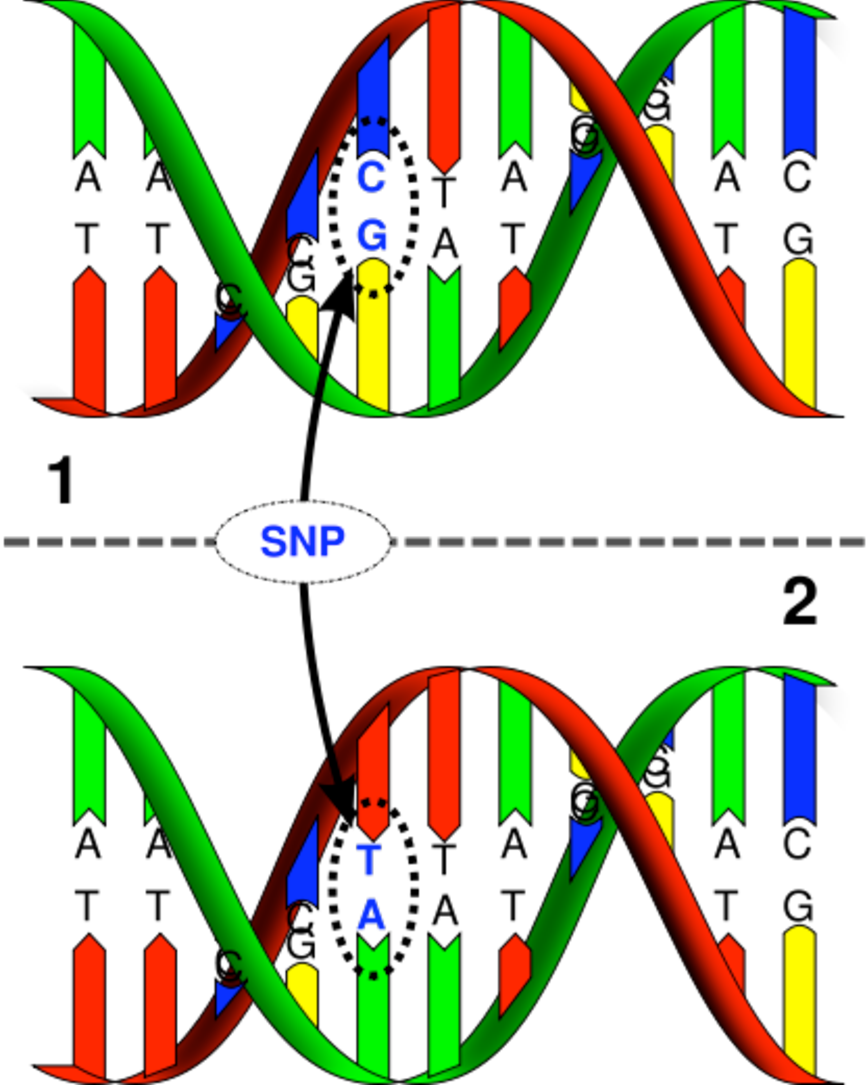
\includegraphics[width=.35\linewidth]{snp.pdf} 
\hspace{2cm}
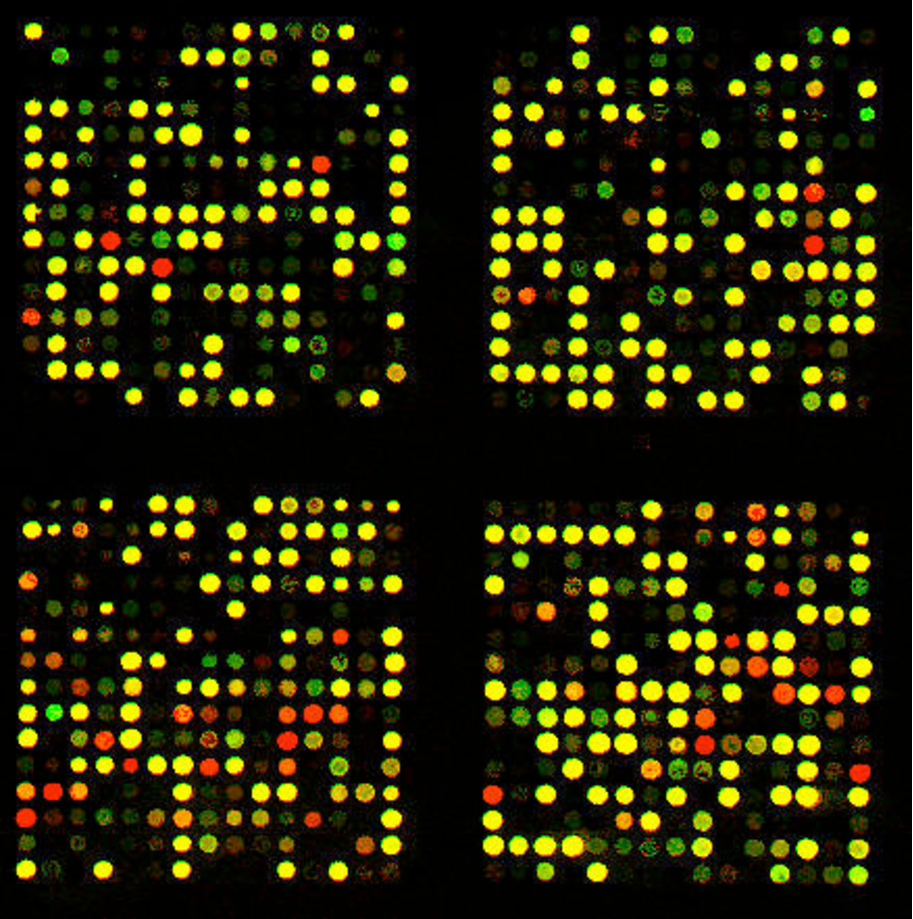
\includegraphics[width=.35\linewidth]{microarray.pdf} 
\end{frame}


\begin{frame}[fragile] 
\frametitle{SNPs}

\begin{itemize}
  \item cubren el genoma (1 SNP/Kb se distribuyen uniformemente)
  \item son la variante estructural mas com\'un 
 \item en total acumulan gran cantidad de variabilidad gen\'etica 
\end{itemize}

Su estudio a nivel individual, local y global es esencial para entender procesos genómicos
\end{frame}

\begin{frame}[fragile] 
\frametitle{SNPs}

Como estructura: 

\begin{itemize}
  \item si affectan funci\'on: eQTLs (expresi\'on), mQTLs (metilaci\'on)
  \item si estan relacionados con enfermedades heredables: SNPs de riezgo 
  \item o pueden estar bajo presiones evolutivas  
  \item o pueden no hacer nada ... (mendelian randomization)
\end{itemize}

\end{frame}


\begin{frame}[fragile] 
\frametitle{SNPs}
Propiedades:

\begin{itemize}
  \item Mutaciones Mendelianas
  \item Taza de mutaci\'on $10^8$ generaciones
  \item Sometidos a deriva gen\'etica, selecci\'on o migraci\'on 
\end{itemize}

\end{frame}


\begin{frame}[fragile] 
\frametitle{SNPs}
Estructura local

\begin{itemize}
  \item Est\'an sometidos a recombinación
  \item Que dos SNPs recombinene depende de su distancia
  \item Por tanto SNPs locales estan correlacionados
\end{itemize}

\end{frame}


\begin{frame}[fragile] 
\frametitle{Correlaci\'on entre SNPs}
Estructura local

\begin{itemize}
  \item Est\'an sometidos a recombinación
  \item Que dos SNPs recombinene depende de su distancia
  \item Por tanto SNPs locales estan correlacionados
\end{itemize}
\end{frame}



\begin{frame}[fragile] 
\frametitle{LD}
Estructura local

Correlaci\'on o Linkage Disequilibrium entre SNPs se mide con 

\begin{table}[]
\centering
\begin{tabular}{c|cc|c}
  & A & T &  Total \\ \hline
C &  $x_{CA}$  &  $x_{CT}$  &  $q_C$ \\
A &  $x_{AA}$  &  $x_{AT}$  &  $q_A$  \\ \hline
Total & $p_A$  &  $p_T$  &   1 \\
\end{tabular}
\end{table}
Lo que se desvían las casillas de la asociaci\'on por azar:
$D=p_A*q_C - x_{CA}$ o $D=-p_C*q_T + x_{CT}$, ...
\end{frame}


\begin{frame}[fragile] 
\frametitle{LD}
SNPs se genotipan individualmente por lo que la fase se pierde! 

\begin{table}[]
\centering
\begin{tabular}{c|ccc|c}
 & A/A=0 & A/T=1 & T/T=2 &  Total \\ \hline
C/C=0 &  $y_{00}$  &  $y_{01}$ & $y_{02}$ & $q_0^2$ \\
C/A=1 &  $y_{10}$  &  $y_{11}$ & $y_{12}$ & $2*q_0*q_1$  \\ 
A/A=2 &  $y_{20}$  &  $y_{21}$ & $y_{22}$ & $q_1^2$  \\ \hline
Total & $p_0^2$  &  $2*p_0*p_1$  & $p_1^2$ &   1 \\
\end{tabular}
\end{table}
$x_{CA} =2*y_{00} + y_{01} + y_{10} +n*y_{11}$, n? 
\end{frame}


\begin{frame}[fragile] 
\frametitle{Fase}

Un sujetos en $y_{11}$ puede ser 

\begin{table}[]
\centering
\begin{tabular}{ccccc}
      &SNP1& &SNP2 & \\
chr1: &C   &-&  A& (S\'i est\'a en $x_{CA}$)\\
chr2: &A   &-&  T& o \\
& & & &\\ \hline
chr1: &C   &-&  T& (No est\'a en $x_{CA}$)\\
chr2: &A   &-&  A&  \\
\end{tabular}
\end{table}

Si se conoce la fase se conocen los haplotipos, regiones donde el LD es alto
\end{frame}


\begin{frame}[fragile] 
\frametitle{Regiones con LD alto}

Las regiones con LD alto dependen de la ancestr\'ia.
$r^2$ es una medida normalizada de $D$. $r^2=D^2/(p_A*p_T*q_C*q_A)$

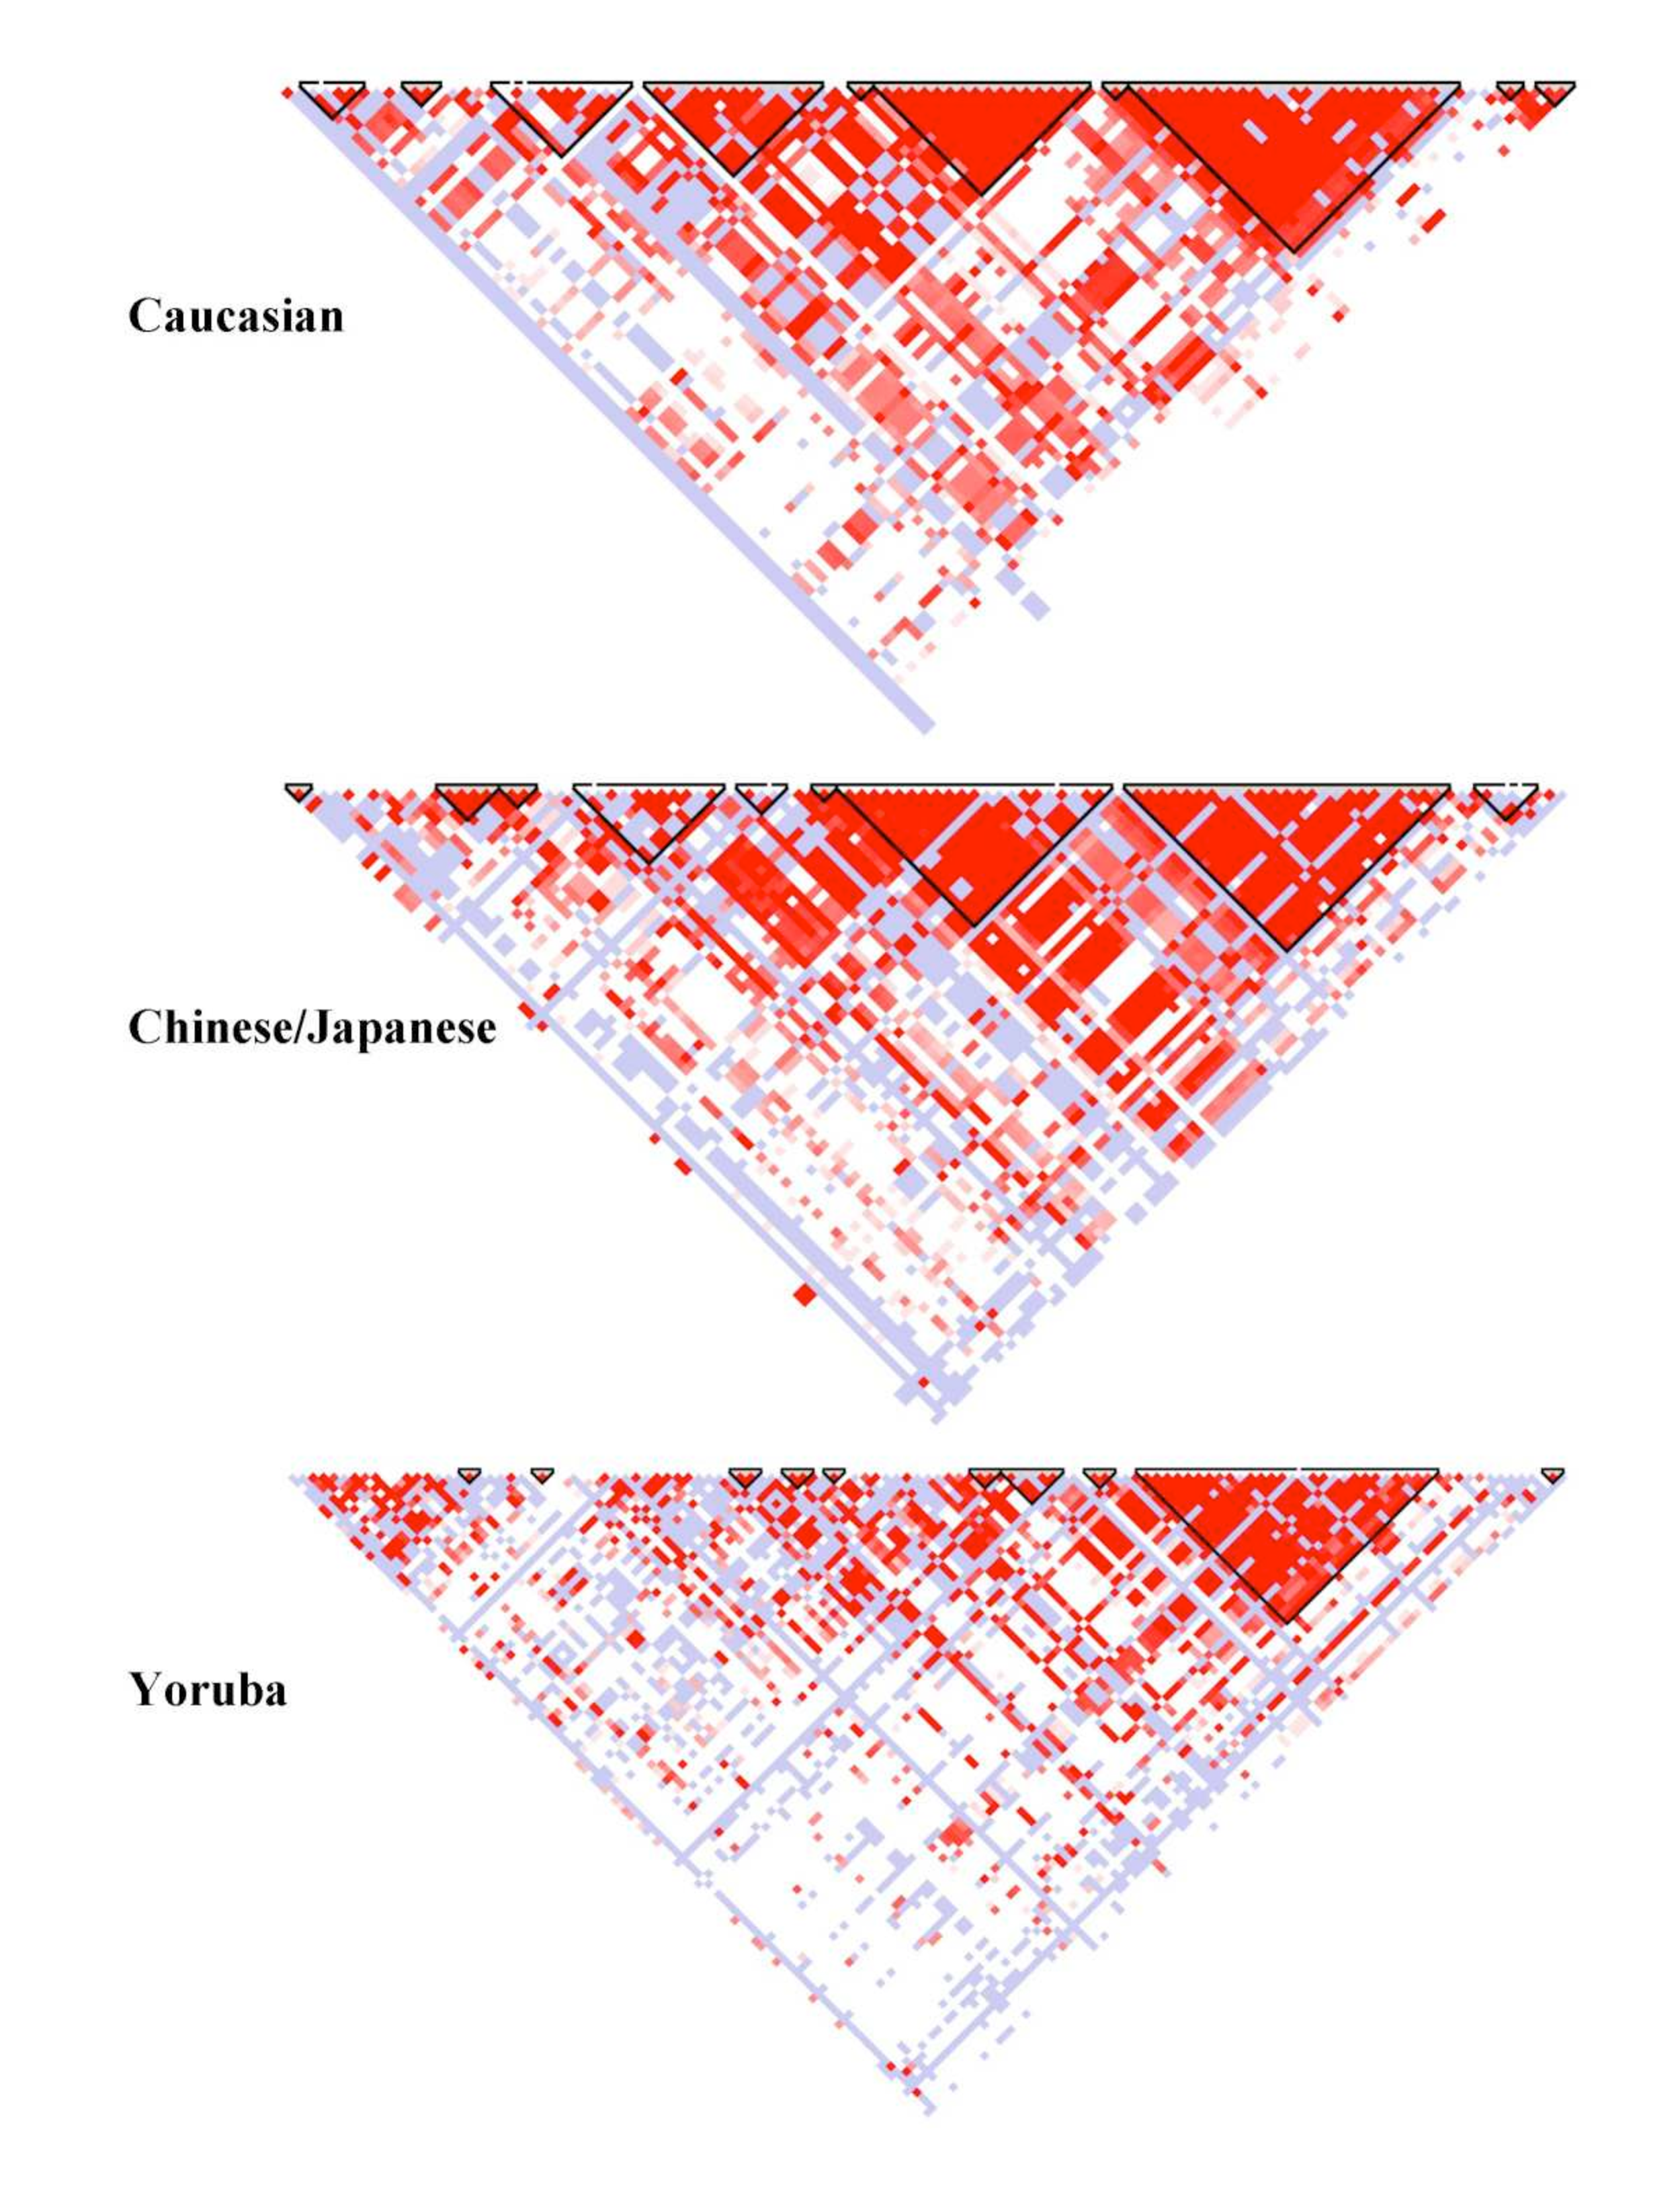
\includegraphics[width=.5\linewidth]{mozscreenshot141.pdf}
\end{frame}


\begin{frame}[fragile] 
\frametitle{LD con distancia}
La recombinaci\'on disminuye el LD y aumenta con la distancia entre SNPs.
Hay regiones con muchos SNPs que tienen LD alto entre ellos

\vspace{2cm}
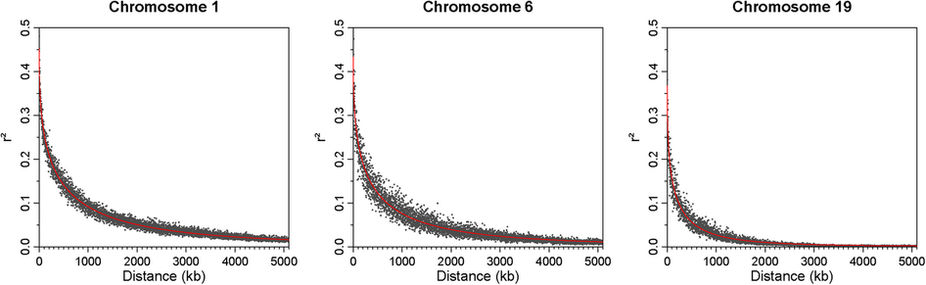
\includegraphics[width=1\linewidth]{LDdistance.jpg}

\end{frame}

\begin{frame}[fragile] 
\frametitle{Haplotipos}

Esas regiones forman haplotipos frequentes: 
macroestructuras de SNPs correlacionados.

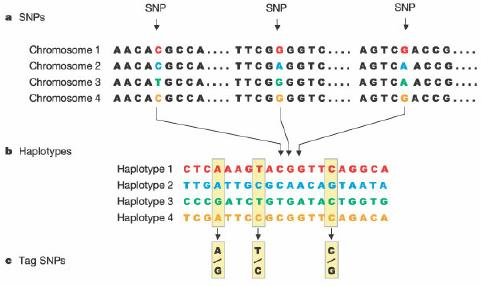
\includegraphics[width=0.8\linewidth]{haplo.jpg}

\end{frame}


\begin{frame}[fragile] 
\frametitle{Hapotipos}

Los haplotipos son la principal estructura que generan los SNPs
Son indicativos de
\begin{itemize}
\item historia evolutiva: haplotipos en EU son mas grandes que en AF
\item patrones especificos de recombinacion: Diferencias en hotspots
\item presencia de otros variantes etructurales que repimen la recombinacion.
\end{itemize}

\end{frame}


\begin{frame}[fragile] 
\frametitle{Hapotipos}

``Si se conocen los haplotipos mas frecuentes de una poblaci\'on
entonces pocos SNPs pueden taggear los haplotipos''

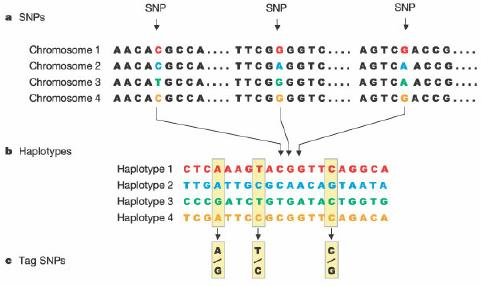
\includegraphics[width=0.8\linewidth]{haplo.jpg}

\end{frame}



\begin{frame}[fragile] 
\frametitle{Hapotipos}

Si tenemos los haplotipos de referencia de una poblaci\'on
\begin{itemize}
\item Podemos predecir los SNPs no genotipados (imputar)
\item Podemos encontrar una asociacion funcional en regiones alrededor de un SNP causal
\item No hay que genotiparlos todos los SNPs
\end{itemize}

sin embargo
\begin{itemize}
\item no tendremos infomaci\'on sobre variantes mas raras u espec\'ificas
\item cada poblaci\'on tiene una historia evolutiva diferente
\end{itemize}

\end{frame}



\begin{frame}[fragile] 
\frametitle{T\'ecnicas de genotipaci\'on}

Secuenciaci\'on
\begin{itemize}
\item los SNPs son variantes estructurales por lo que la secuenciación es método ideal
\item es cara y estudios de cohortes son hoy en dia impensables
\end{itemize}

hibridaci\'on
\begin{itemize}
\item se pueden sintetizar millones de sondas fluoresentes y ponerlas en un chip (miroarrays)
\item es barato y se puede hacer en miles de individuos
\item hay que conocer que sondas hay que poner
\item las sondas dependen de una poblaci\'on de referencia 
\item no es un metodo para descubrir variantes desconocidas
\end{itemize}

\end{frame}


\begin{frame}[fragile] 
\frametitle{microarrays}

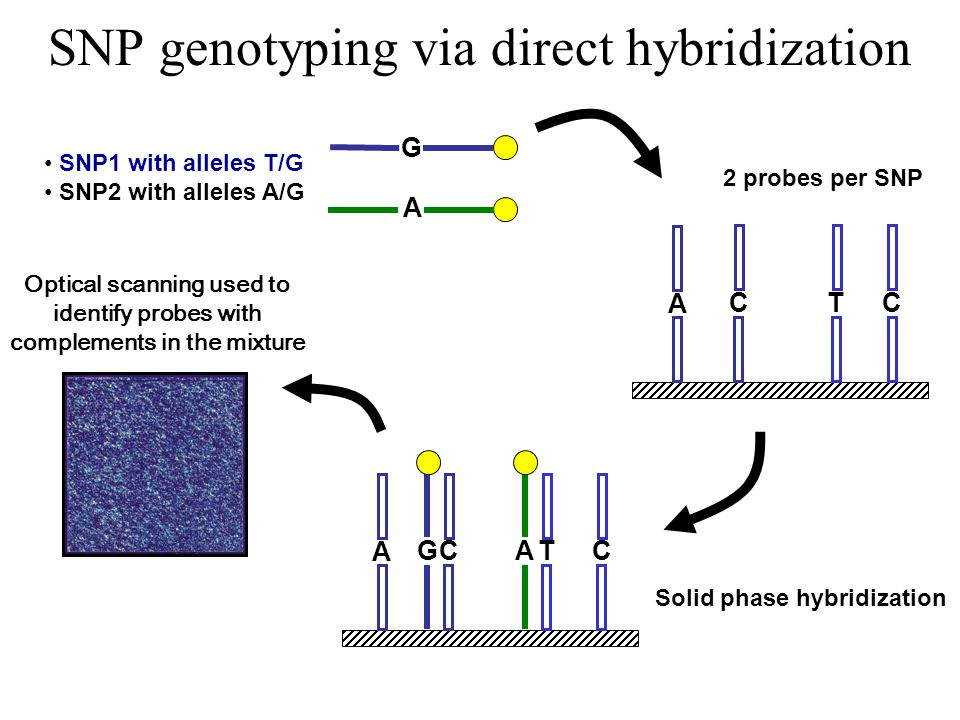
\includegraphics[width=0.8\linewidth]{micro2.jpg}

cada punto es una sonda y el color e intensidad de la luz emitida determina si una muestra hiridiz\'o 

\end{frame}

\begin{frame}[fragile] 
\frametitle{microarrays}

cada sujeto tiene una intensidad for cada alelo(A y B)
\begin{center}
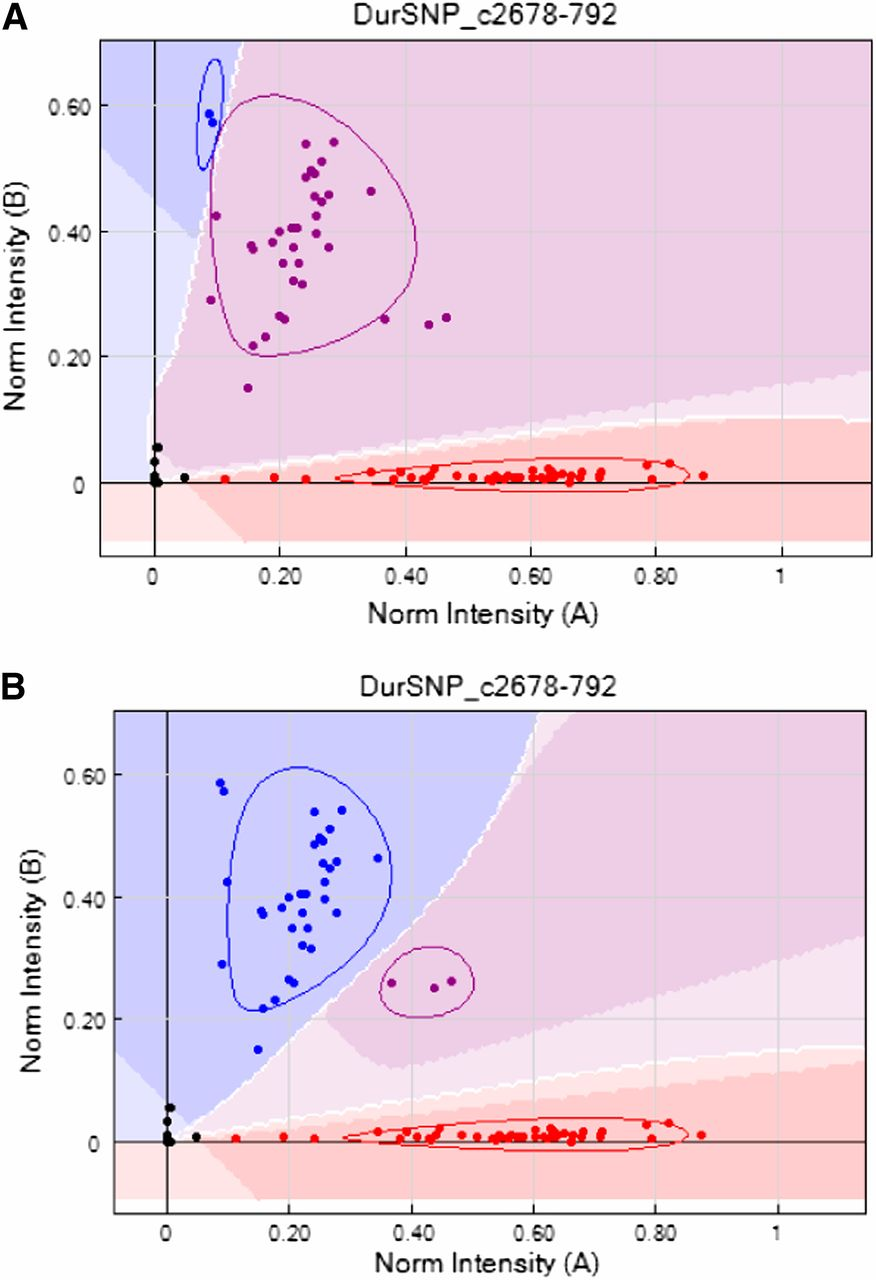
\includegraphics[width=0.3\linewidth]{clustermicro.jpg}
\end{center}
entre menos varianza en angulo entre los grupos mejor es la genotipacion del SNP

\begin{itemize}
\item B-allelefreq: la intensidad relativa del allelo B respecto al A (angulo)
\item log2ratio: la intensidad de la observaci\'on respecto al grupo (magnitud)
\end{itemize}
\end{frame}



\begin{frame}[fragile] 
\frametitle{microarrays}

SNP arrays como medida indirecta de otros variantes estructurales
\begin{center}
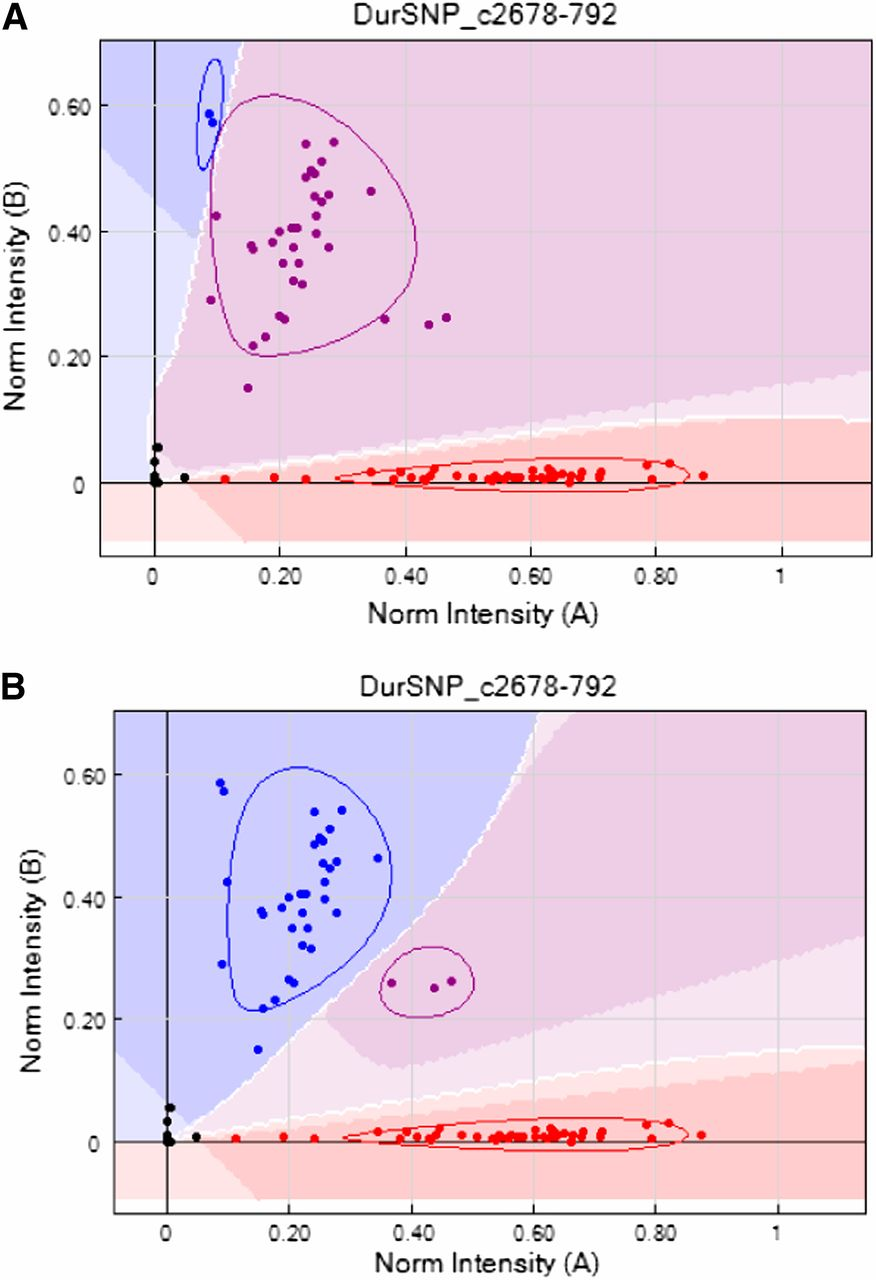
\includegraphics[width=0.3\linewidth]{clustermicro.jpg}
\end{center}

\begin{itemize}
\item B-allelefreq: si un individuo esta entre dos clusters puede que tenda dos genotipos en sus celulas (Mosaicismos) 
\item log2ratio: mas intensidad es indicativo de mas copias de un allelo (CNVs)
\end{itemize}

\end{frame}



\begin{frame}[fragile]
\frametitle{GenomeStudio}
Es el software de Illumina para hacer el genotipado de los SNPs (clustering)
\newline
\begin{center}
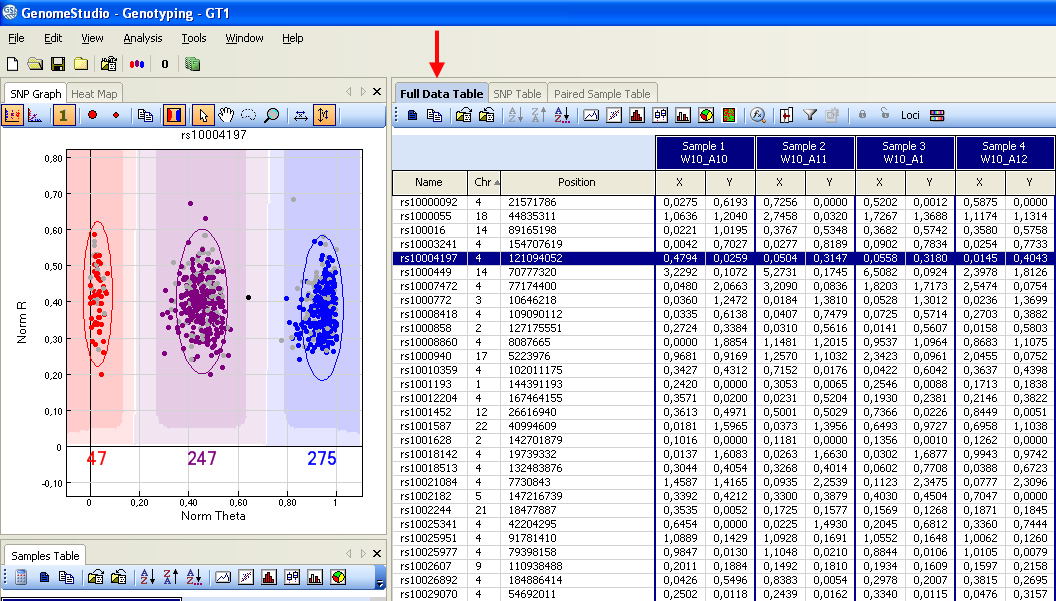
\includegraphics[width=0.5\linewidth]{genomestudio.jpg}
\end{center}

\begin{itemize}
\item produce los genotipos en formato PLINK 
\item datos de B-allele freq y log2ratio son \'utiles para el gentipado de mosaicismos y CNVs (no lo hace GenomeStudio)
\end{itemize}

\end{frame}




\begin{frame}[fragile]
\frametitle{Genome-wide SNPs}
SNPs genome-wide: barrido genomico con alguna resoluci\'on

objetivo: determinar a que cromosoma de un individuo corresponde cada alelo

\begin{itemize}
\item sequencia: ensamblar los reads
\item microarrays: fasearlos 
\end{itemize}
\end{frame}


\begin{frame}[fragile]
\frametitle{Trios}
Los datos de trios ayudan a resolver la fase
\begin{table}[]
\centering
\begin{tabular}{cccccccc}
      &SNP1& &SNP2 & & SNP3 &  & SNP4\\
hijo chr padre: &C   &-&  A/T&-& G &-& G/A\\
hijo chr madre: &C   &-&  A/T&-& G &-& G/A\\ 
& & & &\\
padre chr1: &C/A   &-&  T&-& G/C &-& G/A\\
padre chr2: &C/A   &-&  T&-& G/C &-& G/A\\ 
& & & &\\
madre chr1: &C   &-&  A/T&-& G &-& G/A \\
madre chr2: &C   &-&  A/T&-& G &-& G/A\\ 
& & & &\\
com\'un chr: & C  &-&  T &-& G &-& G\\
menos com\'un chr & C  &-&  T &-& G &-& A\\
\end{tabular}
\end{table}
\end{frame}


\begin{frame}[fragile]
\frametitle{Hapotipos}

Recordemos: Si tenemos los haplotipos de referencia de una poblaci\'on
\begin{itemize}
\item Podemos predecir los SNPs no genotipados (imputar)
\item Podemos encontrar una asociacion funcional en regiones alrededor de un SNP causal
\item No hay que genotiparlos todos los SNPs
\end{itemize}
es una estimaci\'on de la varuiabilidad gen\'etica de la poblaci\'on

\end{frame}


\begin{frame}[fragile]
\frametitle{HAPMAP}
Un proyecto de libre acceso a los datos

\begin{center}
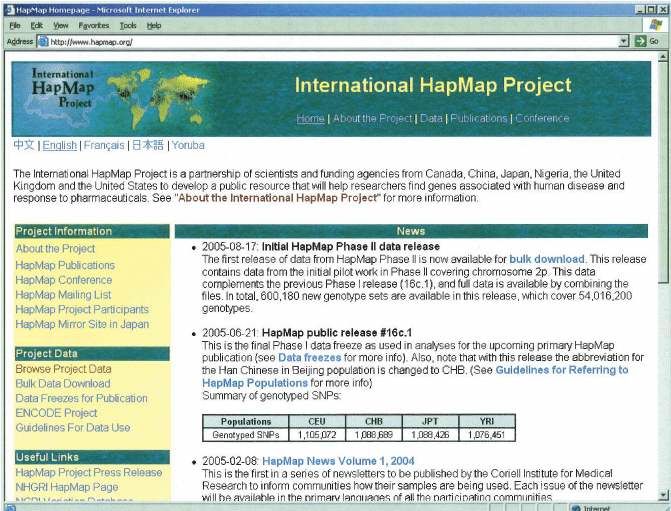
\includegraphics[width=0.5\linewidth]{hapmap.png}
\end{center}

public\'o los \'ultimos datos (fase III) en el 2009.
Loa datos est\'an accesibles en formato PLINK.
\end{frame}




\begin{frame}[fragile]
\frametitle{HAPMAP}
HapMap II
\begin{itemize}
\item     30 tr\'ios (padres e hijo) de Nigeria.
\item     30 tr\'ios de Estados Unidos de origen europeo. 
\item     44 individuos sin relaci\'on gen\'etica de Jap\'on (Tokio).
\item     45 individuos sin parentesco de China (Peking).
\end{itemize}

HapMap III 
\begin{itemize}
\item se extendio a 11 poblaciones diferentes inlcuyendo mas africanos, indios y mexicanos.
\item Abarca unos 2 Millones de SNPs
\end{itemize}

\end{frame}


\begin{frame}[fragile]
\frametitle{1000 genomes}

\begin{center}
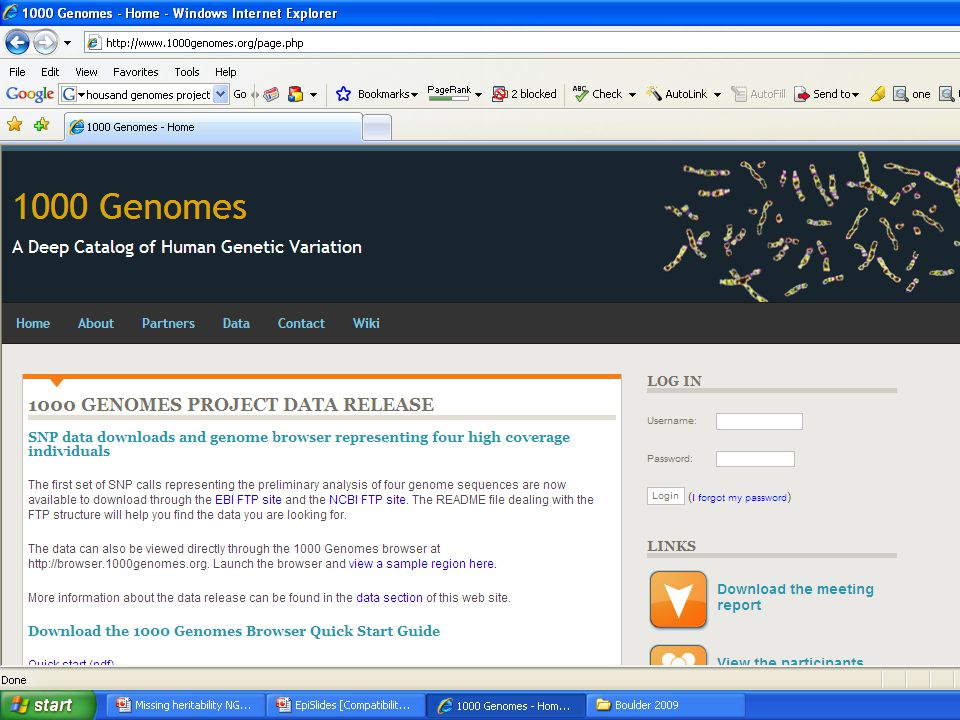
\includegraphics[width=0.5\linewidth]{1kG.jpg}
\end{center}
\end{frame}


\begin{frame}[fragile]
\frametitle{1000 Genomas}

R\'apidamente HapMap fue remplazado por los 1000 Genomas
\begin{itemize}
\item     secuenciaci\'on de 1092 individuos
\item     26 poblaciones 
\item     36 Millones de SNPs 
\item     los datos est\'an accesibles en formato VCF 
\item     est\'an integrados con el Genome Browser 
\end{itemize}

\end{frame}


\begin{frame}[fragile]
\frametitle{1000 Genomes}

\begin{center}
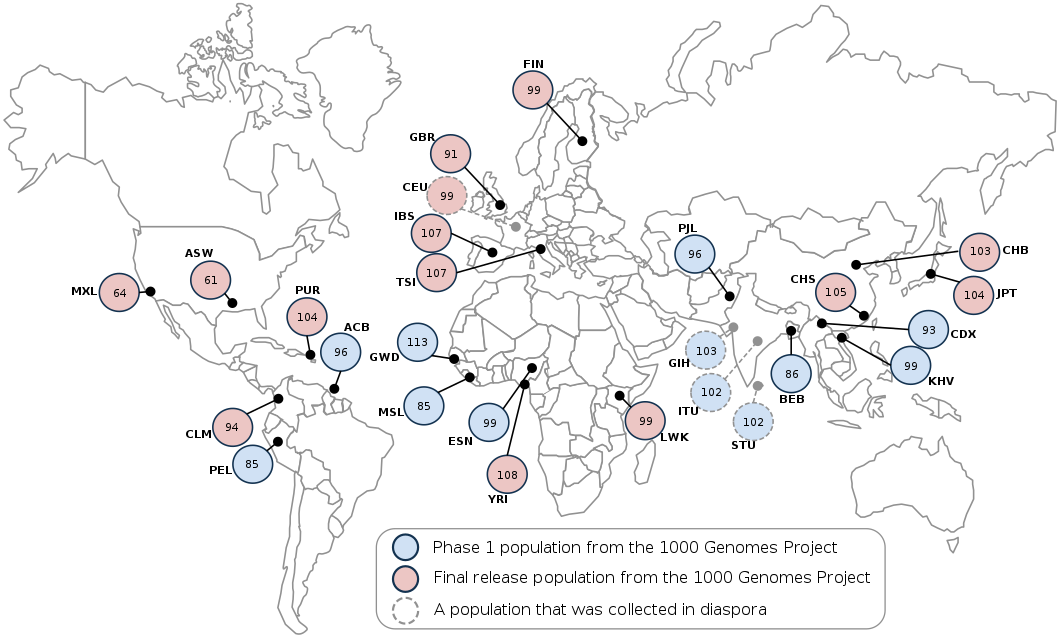
\includegraphics[width=0.5\linewidth]{1000_Genomes.png}
\end{center}
Datos publicados el 2012
\end{frame}

\begin{frame}[fragile]
\frametitle{Otros proyectos}

\begin{itemize}
\item     100 000 Genomes lanzado el 2014 (UK)
\item     Simons genome diversity proyect 300 individuos de 142 poblaciones lanzado 2016
\item     The haplotye reference consortium 
\end{itemize}

\end{frame}

\begin{frame}[fragile]
\frametitle{The haplotye reference consortium}

\begin{itemize}
\item     100 000 Genomes lanzado el 2014 (UK)
\item     Simons genome diversity proyect 300 individuos de 142 poblaciones lanzado 2016
\item     The haplotye reference consortium  64,976 individuos 39Millones de SNPs
\end{itemize}

\end{frame}

\begin{frame}[fragile]
\frametitle{The haplotye reference consortium}

\begin{center}
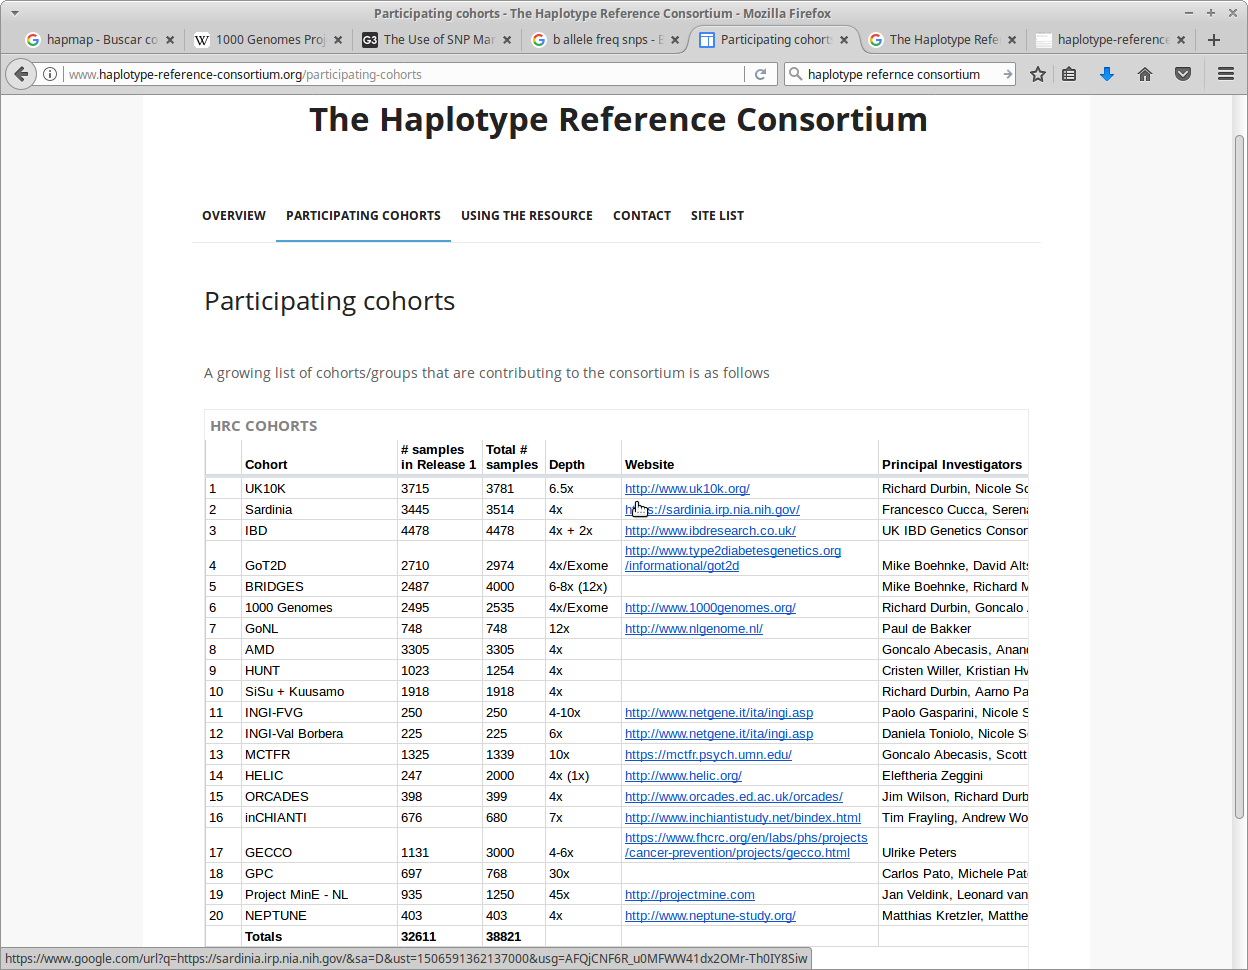
\includegraphics[width=0.5\linewidth]{haplotref.png}
\end{center}
Datos publicados el 2012
\end{frame}


\begin{frame}[fragile]
\frametitle{Haplotipos de referencia}

Una vez identificados los haplotipos de referencia
\begin{itemize}
\item variabilidda gen\'etica de la poblaci\'on
\item frecuencia de alelos funcionales
\item frecuencia de alelos de riezgo
\end{itemize}

\end{frame}

\begin{frame}[fragile]
\frametitle{Variabilidad gen\'etica}

La variabilidad g\'enetica dada por los haplotipos de referencia contribuye a determinar:

\begin{itemize}
\item la especificidad y frequencia de haplotipos 
\item medidas globales de heterocigocidad 
\item medidas globales de fijacion (FST)
\item patrones de recombiaci\'on
\item la presencia de otras variantes gen\'eticas (CNVs, mosaicismos o inversiones)
\end{itemize}
\end{frame}


\begin{frame}[fragile]
\frametitle{Variabilidad gen\'etica}
estudios comparativos permite estudiar
\begin{itemize}
\item la distancia gen\'etica a otras poblaciones 
\item evidencia de selecci\'on en regiones particulares
\item evidencia de patrones de migracion y mestizage
\end{itemize}
\end{frame}


\begin{frame}[fragile]
\frametitle{Variabilidad gen\'etica}
estudios comparativos permite estudiar
\begin{itemize}
\item la distancia gen\'etica a otras poblaciones 
\item evidencia de selecci\'on en regiones particulares
\item evidencia de patrones de migraci\'on y mestizage
\end{itemize}
\end{frame}



\begin{frame}[fragile]
\frametitle{Estudios de asociaci\'on gen\'etica}
Tener un panel de referencia permite
\begin{itemize}
\item estimar las frecuencias que se esperan en la poblaci\'on general 
\item tener un grupo ''control´´
\item estudiar el contexto gen\'etico de los efectos de un SNP de riezgo
\item integrar estudios de asociacion gen\'etica (imputaci\'on)
\end{itemize}
\end{frame}



\begin{frame}[fragile]
\frametitle{Estudios de asociaci\'on gen\'etica}

Los GWAS pretenden encontrar los SNPs de riezgo a una enfermedad (caracter\'istica heredable)

\begin{center}
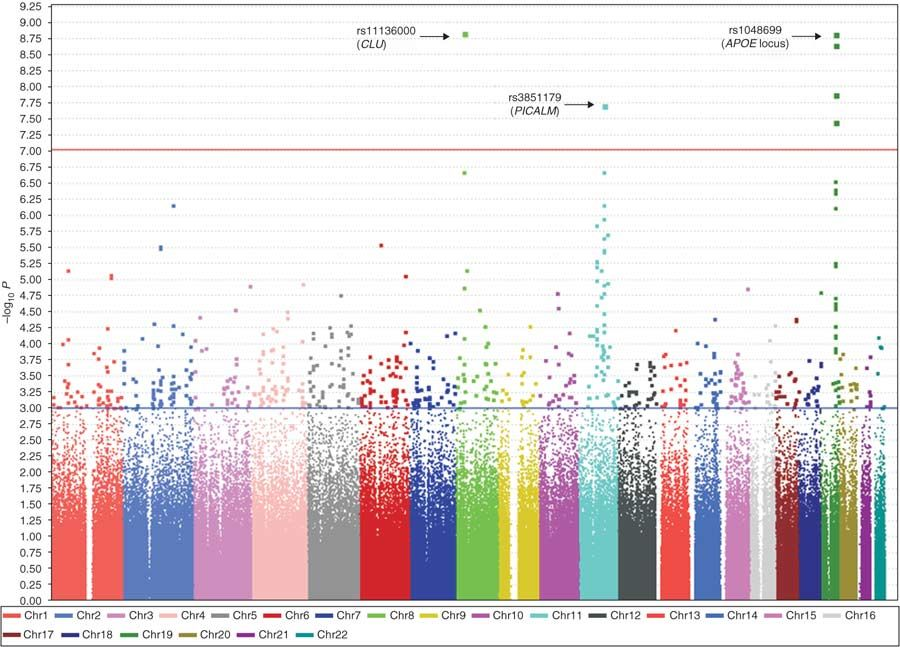
\includegraphics[width=0.5\linewidth]{alz.jpg}
\end{center}

Se basan en la hipotesis de que enfermedades comumunes pueden ser explicadas por variantes comunes
\end{frame}


\begin{frame}[fragile]
\frametitle{Estudios de asociaci\'on gen\'etica}

Los GWAS pretenden encontrar los SNPs de riezgo a una enfermedad (caracter\'istica heredable)

\begin{center}
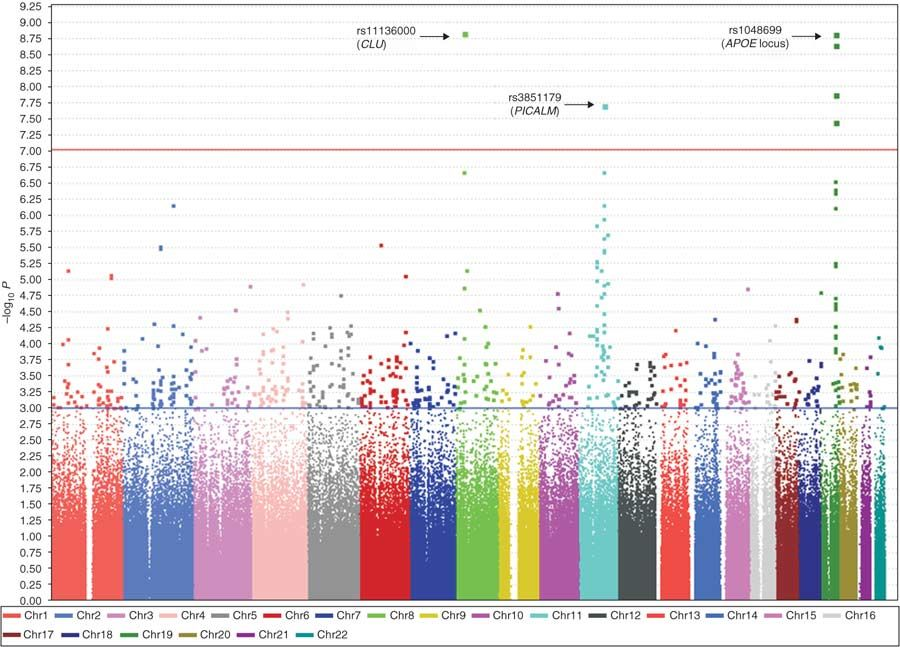
\includegraphics[width=0.5\linewidth]{alz.jpg}
\end{center}

Se basan en la hip\'otesis de que enfermedades comumunes pueden ser explicadas por variantes comunes
\end{frame}


\begin{frame}[fragile]
\frametitle{Estudios de asociaci\'on gen\'etica}

Hay miles de estudios reportados
\begin{center}
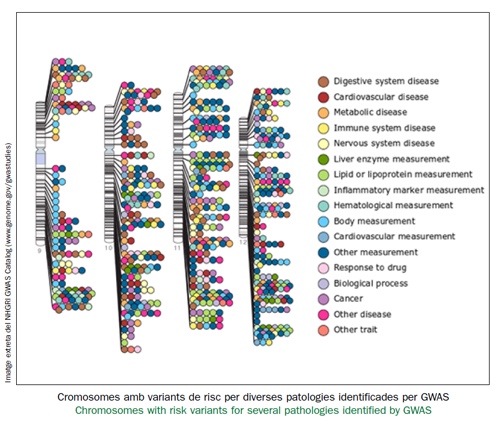
\includegraphics[width=0.5\linewidth]{gwascat.jpg}
\end{center}
\end{frame}


\begin{frame}[fragile]
\frametitle{Estudios de asociaci\'on gen\'etica}

Se encuentran muchos efectos pequeños aditivos por lo que es necesario grandes estudios 
\begin{center}
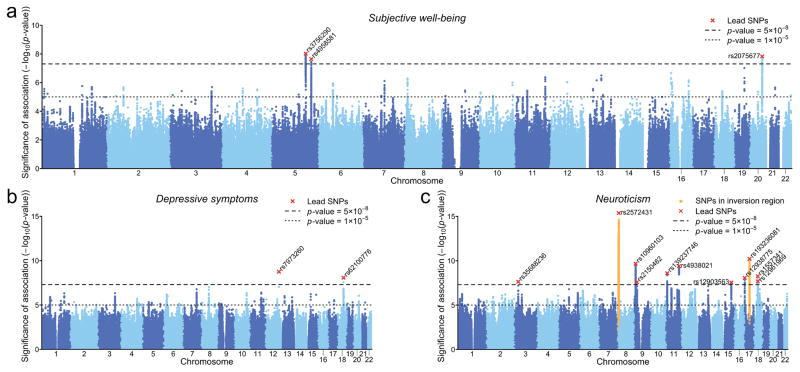
\includegraphics[width=0.7\linewidth]{neurotic.jpg}
\end{center}

\begin{itemize}
\item  298,420 sujetos para sintomas de bienestar
\item  161,460 sujetos para sintomas de depresi\'on
\item  170,910 sujetos para sintomas de neuroticismo
\end{itemize}
\end{frame}



\begin{frame}[fragile]
\frametitle{Estudios de asociaci\'on gen\'etica}
Cada cohorte tiene unos datos de SNPs particulares, difrente densidad de SNPs.
\begin{itemize}
\item  la imputaci\'on de los datos es necesaria para integrar las cohortes
\item  la imputaci\'on depende de los haplotipos de referencia
\end{itemize}
\end{frame}



\begin{frame}[fragile]
\frametitle{Haplotipos de referencia Colombianos}

Variabilidad gen\'etica
\begin{itemize}
\item  estructura de los haplotipos por regiones
\item  diferencias con haplotipos en otras poblaciones globales
\item  estructura de los haplotipos mestizos
\item  haplotipos indigenas
\item  los puntos de recombinaci\'on son facilmente identificables 
\item  effectos de migraci\'on
\item  señales de selecci\'on
\item  frequencia de otros variantes estructurales
\end{itemize}

\end{frame}


\begin{frame}[fragile]
\frametitle{Haplotipos de referencia Colombianos}
A nivel de SNPs
\begin{itemize}
\item  frecuencia de SNPs de riezgo en poblaci\'on general
\item  effectos de SNPs en un contexto de mestizage
\item  cambios funcionales
\item  cambios de riezgo a enfermedades
\item  effecto en la interaccion entre SNPs (epistasis)
\end{itemize}
\end{frame}


\begin{frame}[fragile]
\frametitle{Haplotipos de referencia Colombianos}

imputaci\'on
\begin{itemize}
\item  como se efecta la imputaci\'on al tener haplotipos mestizos
\item  como afecta el faseado al tener una poblaci\'on mestiza
\item  los heplotipos del los 1000 genomas son representativos? 
\end{itemize}
\end{frame}


\end{document}
